\subsection{Analisador sintático e tradutor}
\label{subsec:sintatico:desenho}

Para o analisador sintático, criaram-se algumas estruturas de suporte ao
\emph{parser}, nomeadamente uma \emph{hashtable} para a tabela de
identificadores, uma biblioteca para os dados referentes a cada identificador,
uma biblioteca para suporte ao \emph{parser}, com toda a informação relativa ao
estado do \emph{parser}-- apontador de endereços na \emph{stack} virtual,
\emph{stacks} para calculo do nível das \emph{etiquetas}-- e, adicionalmente
definiram-se tipos enumerados para serem usados em transversalmente na
aplicação.





\subsubsection{Estruturas de dados}
\label{subsec:subsubsec:estruturas:desenho}

A biblioteca \texttt{entry} possui uma estrutura composta pelos campos
mencionados em secções anteriores: tipo, classe, nível, que são tipos
enumerados, e, endereço base, número de linhas máximo (caso seja uma matriz
) e tamanho máximo (para \emph{arrays} unidimensionais e bidimensionais).
Adicionalmente, considerou-se a criação de uma lista de argumentos, no entanto,
por razões que serão posteriormente explicitadas, decidiu-se não se incluir.

As funções referentes à esta biblioteca, inicializam e desalocam memória e vão
buscar os dados da estrutura, ou atualizam os dados desta estrutura. Para
facilitar a criação de entradas na tabela, com diferentes tipos de classes
(\emph{array}, \emph{matriz} e variável), criaram-se métodos que providenciam
a criação da entrada por classe.


A biblioteca \texttt{program\_status} que guarda informação sobre
o \emph{parsing} tem o formato que se segue;  

\begin{verbatim}
typedef struct stat
{
    char label              [MAX_CONDITION_ROW] [ MAX_LABEL ];
    int  label_stack        [MAX_CONDITION_ROW] [ MAX_LABEL_STACK ];
    int  label_number_size  [MAX_CONDITION_ROW] [ MAX_LABEL_STACK ];
    int spointer            [MAX_CONDITION_ROW] [1];
    int strpointer          [MAX_CONDITION_ROW] [1];
    int size_label_string   [MAX_CONDITION_ROW] [1];
    int addresspointer;
} Program_status;
\end{verbatim}

Basicamente, a estrutura possui \emph{arrays} bidimensionais para
a representação das \emph{stacks} das \emph{labels}. Estas têm 4 linhas, ou
seja, uma linha para cada tipo de estrutura de controlo. Deste modo, a variável
\texttt{label} irá guardar a concatenação dos valores dos níveis de aninhamento,
a variável \texttt{label\_stack} possuirá os contadores para cada nível de
aninhamento e a variável \texttt{label\_number\_size} irá guardar o tamanho da
da \emph{string} resultante do valor de cada nível concatenado. A biblioteca
possui funções comuns às \emph{stacks}, como \texttt{pop}, \texttt{push},
\texttt{top} e, adicionalmente possui funções específicas para a manipulação da
informação das \emph{stacks}, que usa o tipo enumerado
\texttt{CompoundInstruction} para aceder por índice às \emph{stacks}.   

As funções específicas para o cálculo das etiquetas são:

\begin{itemize}
	\item \verb|reset_label_stack|
		Esta função tem por âmbito reinicializar o contador após sair de uma ação 
		semântica, como se poderá ver na secção sobre algoritmos, na posição em 
		\texttt{stack[ stack\_pointer ]}. Note-se que o \texttt{top} é em \texttt{stack
		[stack\_pointer--1 ]} 

  \item \verb|increment_top_label_stack|
		Esta função incrementa o valor do contador na posição \texttt{stack\_pointer
		-1} da \emph{stack} de contadores, ou seja, incrementa uma nova ocorrência
		no mesmo nível.

  \item \verb|char *get_label|              

		Esta função obtém a \emph{string} criada até ao momento, com os valores das
		ocorrências dos níveis concatenados na \emph{string} da \emph{label}.  

  \item \verb|char *push_label|             

		A função \texttt{push\-label} incrementa o valor do \texttt{top} da
		\emph{stack} de contadores,   converte o valor numérico do \texttt{top} para
		uma \emph{string}, calcula o tamanho desta \emph{string} e guarda na
		\emph{stack} de tamanhos das \emph{strings}. Em seguida, concatena
		a \emph{string} convertida `a \emph{string} em construção, sendo esta
		copiada para ser retornada pela função. Adicionalmente, guarda o 
		tamanho da \emph{string} convertida na devida \emph{stack} e avança
		o apontador da \emph{string} em construção por esse tamanho.  

  \item \verb|pop_label|                    

		Obtém o tamanho da \emph{string} concatenada, guardada anteriormente na
		\emph{stack} \texttt{label\_number\_size} e coloca caracteres nulos na pilha
		com a \emph{string} para as \emph{labels}, decrementando o apontador da
		pinha com a \emph{string} no valor desse tamanho. 

\end{itemize}


Note-se que, a descrição desta funções é fundamental para a compreensão do
código, uma vez que serão utilizadas mais adiante no documento.

De igual modo, possui funções para o cálculo de endereços para cada classe de
variável, onde o apontador para a \emph{stack} virtual é incrementado pelo
tamanho da variável.\ Outras funções são a inserção de um identificador com os
seu devidos valores na tabela de identificadores, bem como a procura de um
identificador e remoção de todos os identificadores.\ Por último, a função
\texttt{check\_type} compara dois tipos.\  

Além destas bibliotecas, foram definidos novos tipos, enumerados,  no cabeçalho
\texttt{types.h}, que são os seguintes:


\begin{itemize}
	\item \verb|CompoundInstruction|;
Este tipo carateriza tipos de estruturas de controlo diferentes para acesso por
índice aos \emph{arrays} multidimensionais, representam as diferentes
\emph{stacks} para as \emph{labels}.   

		\begin{itemize}
			\item \texttt{if\_inst}
			\item \texttt{else\_inst}
			\item \texttt{while\_inst}
			\item \texttt{do\_while\_inst}
		\end{itemize}
	\item \verb|Class|;a
		O tipo \texttt{Class} serve para diferenciar as categorias, ou classes, de
		objetos que podem ser declarados e invocados.
		\begin{itemize}
			\item \texttt{Variable}
			\item \texttt{Array}
			\item \texttt{Matrix}
			\item \texttt{Function}
			\item \texttt{Procedure}
			\item \texttt{Nothing}
		\end{itemize}
	\item \verb|Level|;
		O nível tem o propósito de diferenciar programas e subprogramas.
		\begin{itemize}
			\item \texttt{Program}
			\item \texttt{Subprogram}
		\end{itemize}
	\item \verb|Type|;
		Os tipos das variáveis e expressões podem ser os seguintes:
		\begin{itemize}
			\item \texttt{Any}
			\item \texttt{Integer}
			\item \texttt{Boolean}
				Embora se possa atribuir o tipo \texttt{Any} a instruções, não existe
				relevância para o fazer. 
		\end{itemize}
\end{itemize}


\subsubsection{Algoritmos}
\label{subsec:subsubsection:algoritmos:desenho}

\begin{figure}[htpb]
	\centering
	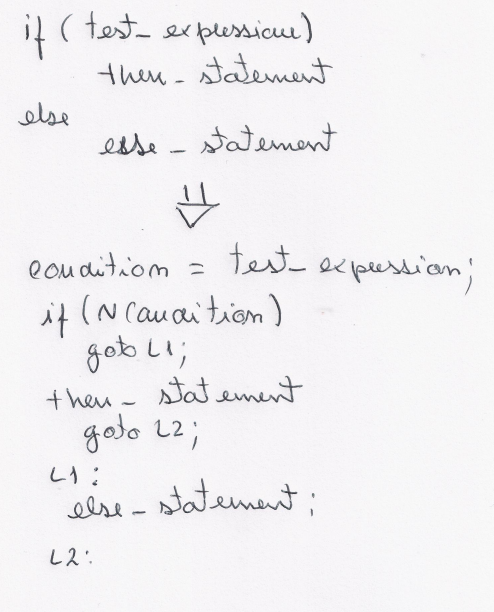
\includegraphics[scale=0.75]{./report/img/ifelse.png}
	\caption{Algoritmo para \texttt{if else}}
\label{fig:figure1}
\end{figure}


\begin{figure}[htpb]
	\centering
	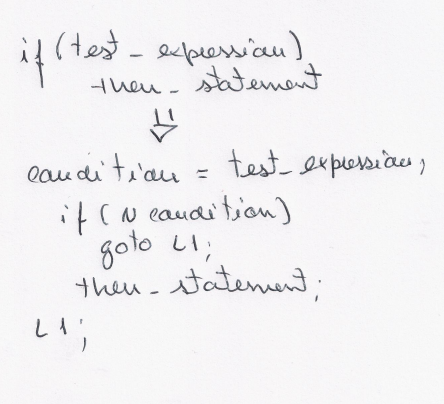
\includegraphics[scale=0.75]{./report/img/if.png}
	\caption{Algoritmo para \texttt{if}}
\label{fig:figure1}
\end{figure}


\begin{figure}[htpb]
	\centering
	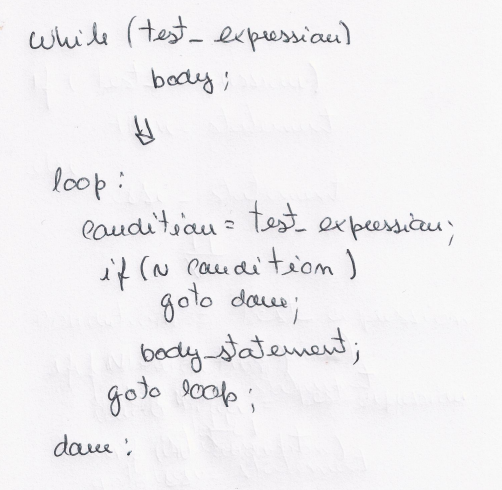
\includegraphics[scale=0.75]{./report/img/while.png}
	\caption{Algoritmo para ciclo \texttt{while}}
\label{fig:figure1}
\end{figure}


\begin{figure}[<+htpb+>]
	\centering
	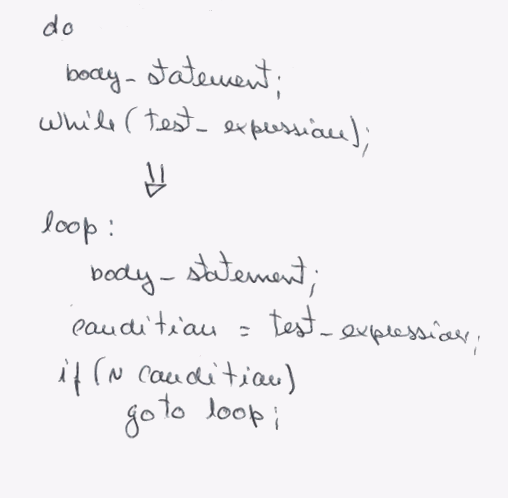
\includegraphics[scale=0.75]{./report/img/dowhile.png}
	\caption{Algoritmo para ciclo \texttt{do while}}
\label{fig:figure1}
\end{figure}






\url{http://lh3lh3.users.sourceforge.net/udb.shtml.}
